23. $|x|\cdot\cfrac{x^3-x^2-x+1}{x^3+x^2-x-1}\geqslant 0\Leftrightarrow|x|\cdot\cfrac{x^2(x-1)-(x-1)}{x^2(x+1)-(x+1)}\geqslant 0\Leftrightarrow
|x|\cdot\cfrac{(x-1)^2(x+1)}{(x-1)(x+1)^2}\geqslant 0.$
Применив метод интервалов, найдём ответ:
\begin{figure}[ht!]
\center{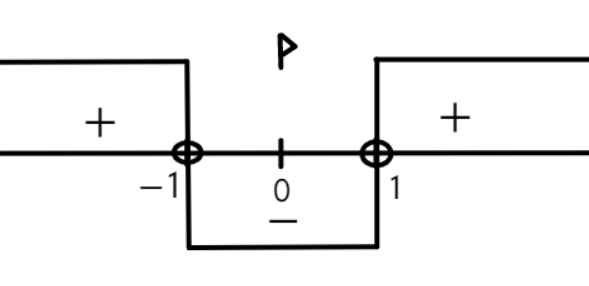
\includegraphics[scale=0.35]{int22.png}}
\end{figure}
$x\in(-\infty;-1)\cup\{0\}\cup(1;+\infty).$\\
